\documentclass{imammb}
\jno{dqnxxx}

\usepackage{natbib, graphicx, amsmath, amsthm, bm, mathrsfs, hyperref}
\hypersetup{colorlinks,citecolor=black,filecolor=black,linkcolor=black,urlcolor=black}

\renewcommand{\theequation}{\thesection.\arabic{equation}}
\numberwithin{equation}{section}
\def\citeasnoun{\cite}

\begin{document}

\title{A Model of Individual BMI Trajectories}
\author{ {\sc Laurens Bogaardt, Anoukh van Giessen, H. Susan J. Picavet and Hendriek C. Boshuizen}\\[2pt]
National Institute for Public Health and the Environment (RIVM),\\
Antonie van Leeuwenhoeklaan 9, 3721MA Bilthoven, The Netherlands.\\[6pt]
{\rm [Received on 20 January 2023, Revised on 24 September 2023]}\vspace*{6pt}}
\pagestyle{headings}
\markboth{L. BOGAARDT, A. VAN GIESSEN, H.S.J. PICAVET \& H.C. BOSHUIZEN}{\rm A MODEL OF INDIVIDUAL BMI TRAJECTORIES}
\maketitle

\begin{abstract}
{A risk factor model of BMI is an important building block of health simulations aimed at estimating government policy effects with regard to overweight and obesity. We created a model which generates representative population level distributions and which also mimics realistic BMI trajectories at an individual level so that policies aimed at individuals can be simulated. The model is constructed by combining several datasets. First, the population level distribution is extracted from a large, cross-sectional dataset. The trend in this distribution is estimated from historical data. In addition, longitudinal data are used to model how individuals move along typical trajectories over time. The model faithfully describes the population level distribution of BMI, stratified by sex, level of education and age. It is able to generate life course trajectories for individuals which seem plausible, but it does not capture extreme fluctuations, such as rapid weight loss.}
{micro-simulation, risk factor, BMI, life course, individual trajectories}
\end{abstract}

\subsubsection*{\textit{Acknowledgments}}
The LISS panel data were collected by CentERdata (Tilburg University, The Netherlands) through its MESS project funded by the Netherlands Organization for Scientific Research.

\section{Introduction}

Overweight and obesity pose significant health risks in many countries~\citep{Dai2020}. The link between a high body mass index (BMI) and various health outcomes, including diabetes and cardiovascular disease, has been well established~\citep{Murray2020}. Consequently, governments spend much effort to curb the increasing trends~\citep{VWS2018, VanRinsum2018}. Investigating what course of action is most fruitful is often done using health simulations~\citep{Levy2011}. A risk factor model of BMI is the first building block of such analyses.

In a health simulation, the evolution of a population is simulated and the outcome of a baseline scenario is compared to the outcome of an alternative scenario in which some preventive intervention has taken place. It usually starts with a population described by means of a set of characteristics like sex, age and some risk factor, such as BMI. Relevant diseases are also included. The population's characteristics are then evolved forward in time where transitions are often encoded by a Markov process, meaning each transition only depends on the current state of the population~\citep{Sonnenberg1993}.

One strategy to define a population is to first divide each variable into discrete categories. For BMI, the categorisation of underweight, normal weight, overweight and obese is typical. For all combinations of the categorised variables, the initial population's prevalence is determined and this list of values is updated each time step. This is called a macro-simulation. When the population is subdivided on multiple characteristics, such as the status of various diseases, the total number of groups grows exponentially. At some point, this leads to computational limitations and it pays to switch to a micro-simulation framework. Here, individuals are sampled from an initial distribution and their set of characteristics is updated each time step, describing a unique life course for each individual~\citep{Levy2011}.

Unlike in a macro-simulation, the values of these life course trajectories in a micro-simulation can be measured on a continuous scale. One commonly used method to ensure all individuals together adhere to the population level distribution is to assign to each individual a percentile score indicating where they lie within the distribution. It is then assumed that this relative position stays fixed, even though the shape of the distribution, and the corresponding value, may change as the individual ages throughout the simulation~\citep{McPherson2007, OECD2019}. A more realistic model can have the relative positions fluctuate over time as well~\citep{Vuik2021}. This is the approach we take to model BMI and figure~\ref{fig:Individual Trajectories} shows a comparison between the resulting life course trajectories.

\vspace{-4mm}

\begin{figure}[!h]
\centering
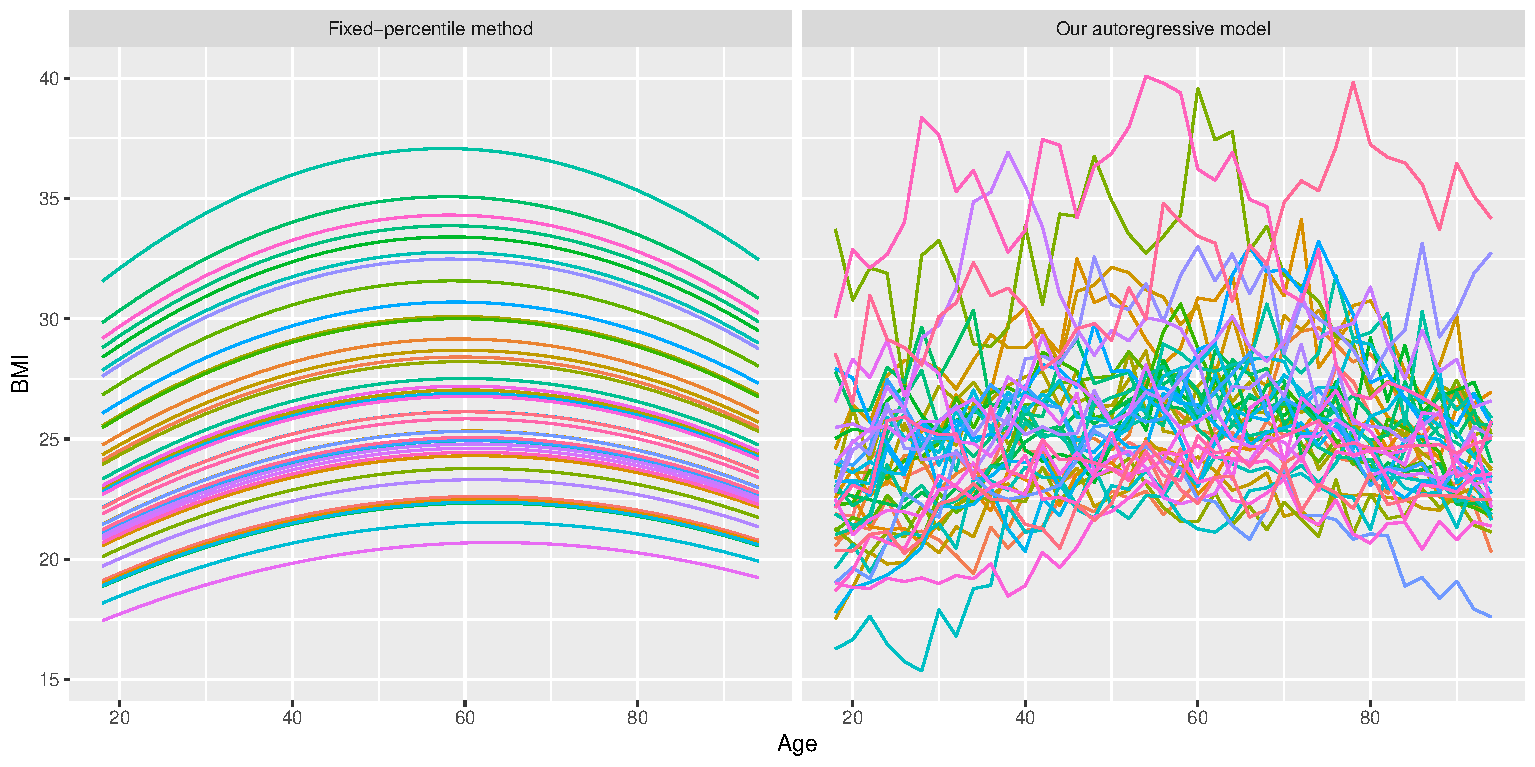
\includegraphics[width=0.96\textwidth] {"Figures/Individual-Trajectories.pdf"}
\vspace*{-2pt}
\caption{A sample of trajectories following the fixed-percentile method compared with those generated by our model.}
\label{fig:Individual Trajectories}
\vspace*{-9pt}
\end{figure}

\vspace{1mm}

In this article, we create a risk factor model of BMI for micro-simulations which is able to faithfully describe the population level distribution, stratified by sex, level of education and age. It can also predict future trends in obesity as well as produce unique life course trajectories for individuals which seem plausible, but it does not capture extreme fluctuations, such as rapid weight loss. It is fit on the adult population of the Netherlands with the purpose of facilitating simulations concerning government policy with regard to overweight and obesity~\citep{TenDam2023}. Although our model serves as a starting point for such analyses by describing the current dynamics of BMI, it makes no claims about the effect of any particular preventive intervention. Our method is simple, tractable and a natural generalisation of the fixed-percentile method. The generic nature means it can be applied to data from various countries and need not be limited to BMI.

To arrive at a realistic and useful BMI model, we would ideally use a large, representative, longitudinal dataset. Unfortunately, longitudinal panels often only include a small number of individuals and most Dutch cohorts are not representative of the population at large. To overcome these limitations, we can cleverly combine a large, cross-sectional dataset with historical- and longitudinal data. The cross-sectional dataset provides representative information about the population level distribution of BMI, described in section~\ref{sec:Population Level Distribution}. In section~\ref{sec:Historical Trend}, we use additional historical data to assess the trend in this distribution. At an individual level, BMI fluctuates over time, following typical trajectories. These trajectories are modelled using the longitudinal data, described in section~\ref{sec:Individual Trajectories}. Finally, in section~\ref{sec:Discussion}, we will discuss some limitations of our model and conclude by suggesting potential future improvements in section~\ref{sec:Conclusion}.

\section{Population Level Distribution}
\label{sec:Population Level Distribution}

\subsection{Approach}
\label{sec:Population Level Distribution/Approach}

We will build up our model of BMI starting with the population level distribution. BMI is defined as body weight divided by the square of height and typical values range between $15 \, kg / m^2$ and $45 \, kg / m^2$. At the population level, its distribution shows positive skew, meaning that it is best modelled by a probability density function flexible enough to deal with non-normal data~\citep{Majer2013}. Although we are modelling the generative process behind BMI, there is no need for a biological interpretation of this process, so any flexible probability density function will do. To fit such a distribution on the adult population of the Netherlands requires a cross-sectional dataset which is representative of the Netherlands. In addition, it must be large enough to accommodate various stratifications. For government policy analyses, stratifying the population by sex, level of education and age is usually adequate. We will develop completely separate models for both sexes, as we believe the differences in biological and environmental influences for males and females warrant distinct models.

\subsection{Data}
\label{sec:Population Level Distribution/Data}

The Public Health Monitor dataset is a Dutch cross-sectional dataset based on a large, health-related questionnaire administered by the Community Health Services, Statistics Netherlands and the National Institute for Public Health and the Environment~\citep{GGD2012}. The dataset contains self-reported weight and height measurements, rounded to nearest kilogram and centimetre. The included survey weights allow for representative analyses of the Netherlands in 2012. The questionnaire was repeated in 2016 and in 2020. However, the data for 2020 are likely to be affected by the COVID pandemic, which is not an effect we would like to include in our model. Furthermore, the data for 2016 will be reserved for external validation, described in the online supplementary information~\citep{Bogaardt2023}. This leads to our choice of fitting the model on the 2012 data.

Table~\ref{tab:Gezondheidsmonitor} provides some descriptive statistics of the variables used which excludes some of the original data, removed in the cleaning process. This is also described in the online supplementary information. Education was measured as the highest level reached and categorised into three levels. The lowest level applies to people with intermediate secondary education or less, the medium level aggregates higher secondary- and intermediate vocational education and highest level includes higher vocational education and university.

\begin{table}[!h]
\tblcaption{Descriptive statistics of the Public Health Monitor dataset.}
{\mbox{\tabcolsep=18pt\begin{tabular}{@{}lcclr@{}}
\tblhead{& Number & Percentage & & Value\\[-9.5pt]}\\[-9.5pt]
Total & 350166 & 100\% & Minimum age & 19.0 \\
Male & 160225 & 45.8\% & Mean age & 56.8 \\
Female & 189941 & 54.2\% & Maximum age & 107.0 \\
Low education & 156041 & 44.6\% & Minimum BMI & 14.0 \\
Medium education & 99302 & 28.4\% & Mean BMI & 25.7 \\
High education & 94823 & 27.1\% & Maximum BMI & 45.0 \lastline
\end{tabular}
\label{tab:Gezondheidsmonitor}
}}
\end{table}

\subsection{Methods}
\label{sec:Population Level Distribution/Methods}

We describe the population level distribution of BMI using the sinh-arcsinh normal distribution~\citep{Jones2009, Jones2019}. It is a variation on the normal distribution following the transformation shown in equation~\ref{eq:Sinh-ArcSinh Transformation}, where $z$ is a normally distributed random variable with zero mean and unit standard deviation. This transformation will also be relevant in section~\ref{sec:Individual Trajectories}, when we apply it to our longitudinal data to turn the BMI values into z-scores. Whenever $\nu = 0$ and $\tau =  1$, a regular normal distribution is obtained where $\mu$ and $\sigma$ control location and scale. Increased values of $\nu$ and $\tau$ result in positive skew and negative kurtosis, respectively.

\vspace{-1mm}

\begin{equation}
\label{eq:Sinh-ArcSinh Transformation}
\text{BMI} \, = \, \mu \, + \, \sigma \times \, \tau \, \times \, \sinh \left(\frac{\text{sinh}^{-1}(z) \, + \, \nu}{\tau}\right)
\end{equation}

\vspace{1mm}

We can incorporate explanatory variables into our analysis by making use of the \textit{GAMLSS} package in R which allows us to model each of the four distribution parameters as functions of the predictors~\citep{Rigby2005, Stasinopoulos2007, R2021}. Initially, we fitted age-dependent splines to all four of the parameters, by sex and level of education. This indicated an approximately quadratic relationship with age for the $\mu$ and $\sigma$ parameters, whereas the level of education mostly impacted their intercept. The $\nu$ and $\tau$ parameters barely differed by age or education. So we repeated the analysis for a restricted, parametric model, given by equation~\ref{eq:Population Level Distribution Parameters}. The limited number of parameters results in a parsimonious model and subsequently makes the application in health simulations easier. The two historical trend coefficients, $\mu_{year}$ and $\sigma_{year}$, are added here for completeness but may be ignored for now; how their values are estimated will be described in section~\ref{sec:Historical Trend}.

\vspace{-1mm}

\begin{equation}
\label{eq:Population Level Distribution Parameters}
\begin{array}{@{\ }rcl@{\ }}
\mu & = & \mu_{education} \, + \, \mu_{age} \, \times \, age \, + \, \mu_{age^2} \, \times \, age^2 \, + \, \mu_{year} \, \times \, year\\
\sigma & = & \sigma_{education} \, + \, \sigma_{age} \, \times \, age \, + \, \sigma_{age^2} \, \times \, age^2 \, + \, \sigma_{year} \, \times \, year \\
\nu & = & \nu_{intercept}\\
\tau & = & \tau_{intercept}
\end{array}
\end{equation}

\vspace{-3mm}

\begin{figure}[!h]
\centering
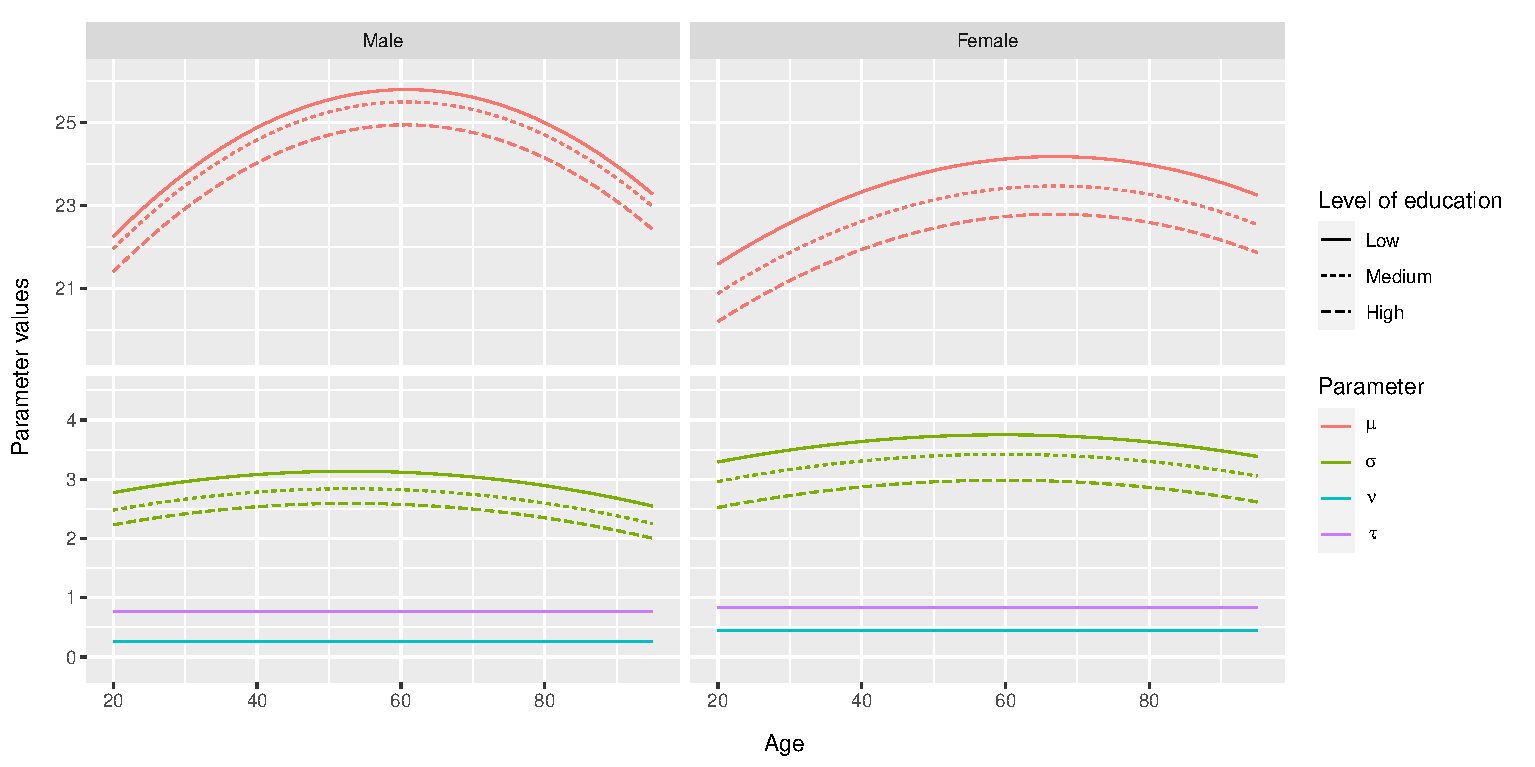
\includegraphics[width=0.99\textwidth] {"Figures/Population-Level-Distribution-Parameters.pdf"}
\caption{The population level distribution parameters for BMI by sex, level of education and age.}
\label{fig:Population Level Distribution Parameters}
\vspace*{-9pt}
\end{figure}

\subsection{Results}
\label{sec:Population Level Distribution/Results}

The resulting parameter values are summarised in figure~\ref{fig:Population Level Distribution Parameters} while the underlying coefficients are listed in the first columns of table~\ref{tab:Population Level Distribution Parameters}. Note again that we are creating separate models for males and females.

\subsection{Internal Validation}
\label{sec:Population Level Distribution/Internal Validation}

To compare the model's predictions and the underlying data, we can categorise BMI into underweight (values below $18.5 \, kg / m^2$), normal weight ($18.5 - 25 \, kg / m^2$), overweight ($25 - 30 \, kg / m^2$) or obese (values of $30 \, kg / m^2$ and above) and determine the observed and modelled prevalences of each of these categories. Figure~\ref{fig:Population Level Prevalences} shows these prevalences, stratified by sex, level of education and age. The model's values are necessarily more smooth due to the low degree of the age polynomial in equation~\ref{eq:Population Level Distribution Parameters}, but the prediction shows good correspondence with the observed data.

\vspace{-3mm}

\begin{figure}[h]
\centering
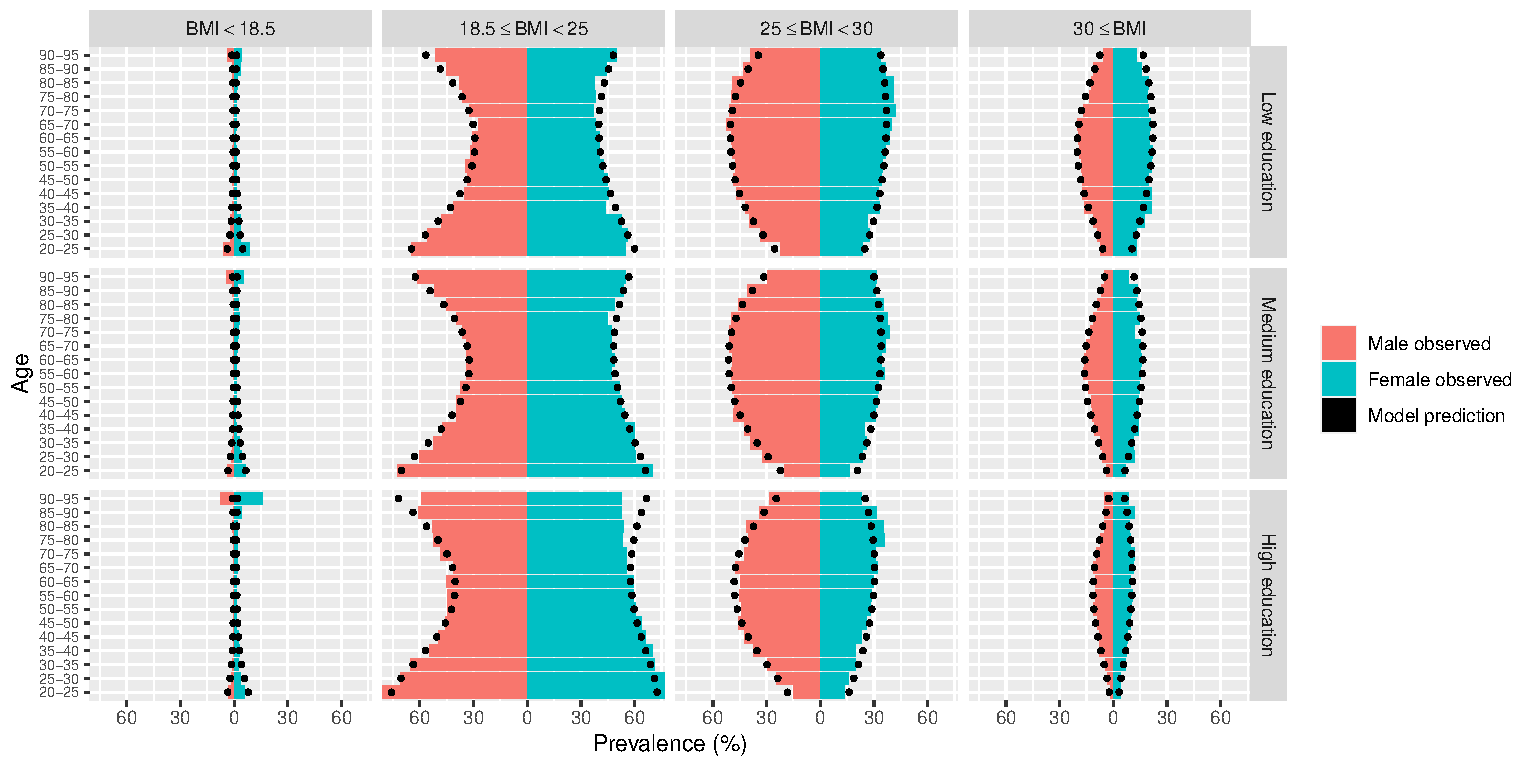
\includegraphics[width=0.99\textwidth] {"Figures/Population-Level-Prevalences.pdf"}
\caption{The observed and modelled prevalences of BMI categories in 2012 by sex, level of education and age.}
\label{fig:Population Level Prevalences}
\vspace*{-9pt}
\end{figure}

\section{Historical Trend}
\label{sec:Historical Trend}

\subsection{Approach}
\label{sec:Historical Trend/Approach}

In this section, we will expand our model by adding a historical trend. In many western countries, including the Netherlands, overweight and obesity have become more prevalent over time. The main drivers are changes in food habits and a more sedentary lifestyle~\citep{Martinez-Gonzalez1999, Swinburn2011, Lopez-Valenciano2020}. Previous work has suggested that this transition increased the spread and skewness of the BMI distribution, rather than solely influencing the mean~\citep{Penman2006, Majer2013, Yamada2020}. Therefore, a linear trend is added to the $\mu$~and~$\sigma$ parameters of the population level distribution, as seen in equation~\ref{eq:Population Level Distribution Parameters}. We will use historical data from the Netherlands to estimate the values of the corresponding $\mu_{year}$ and $\sigma_{year}$ coefficients.

\subsection{Data}
\label{sec:Historical Trend/Data}

Historical data about BMI were assessed by Statistics Netherlands and the National Institute for Public Health and the Environment~\citep{CBS2021}. We use the prevalences of overweight and obesity for adults between 1990 and 2021 which were standardised to the demography of the Netherlands in 2021~\citep{VZinfo2021}. Due to this standardisation step, any trend we extract from these data will mostly be indicative of changes in lifestyle and its influence on BMI rather than also including trends in demography. Table~\ref{tab:VZinfo} shows some of the figures from this dataset.

\begin{table}[!h]
\tblcaption{Historical prevalences of overweight and obesity in the Netherlands.}
{\mbox{\tabcolsep=18pt\begin{tabular}{@{}lcccc@{}}
\tblhead{ \hspace{-4mm} & Overweight males \hspace{-4mm} & Obese males \hspace{-4mm} & Overweight females \hspace{-4mm} & Obese females \\[-9.5pt]}\\[-9.5pt]
1990 & 31.3\% & 5.4\% & 26.7\% & 6.8\% \\
2000 & 35.4\% & 8.3\% & 32.2\% & 9.8\% \\
2010 & 42.3\% & 9.8\% & 30.4\% & 12.5\% \\
2020 & 40.9\% & 12.3\% & 31.5\% & 15.2\% \lastline
\end{tabular}
\label{tab:VZinfo}
}}
\vspace{-2mm}
\end{table}

\subsection{Methods}
\label{sec:Historical Trend/Methods}

To estimate the $\mu_{year}$ and $\sigma_{year}$ coefficients in equation~\ref{eq:Population Level Distribution Parameters} which determine the historical trend, we first realise that if we keep $\nu$ and $\tau$ constant, particular values for $\mu$ and $\sigma$ imply prevalences of overweight and of obesity. Likewise, these prevalences imply values for $\mu$ and $\sigma$. So from the historical prevalences of overweight and obesity in the Netherlands, we can determine how the $\mu$ and $\sigma$ parameter must have changed over time. Subsequently, we perform a linear regression through these values to estimate the $\mu_{year}$ and $\sigma_{year}$ coefficients which best fit the historical data. These coefficients are estimated for males and females separately and are expressed as the change in $\mu$ and $\sigma$ per year relative to 2012, the calibration year of our model. No dependency on the level of education nor on age is included.

\vspace{-1mm}

\subsection{Results}
\label{sec:Historical Trend/Results}

The first part of table~\ref{tab:Population Level Distribution Parameters} lists the coefficients of the population level distribution, previously visualised in figure~\ref{fig:Population Level Distribution Parameters}. The trend coefficients, $\mu_{year}$ and $\sigma_{year}$, are added as the final two columns of this table. Taken together with equations~\ref{eq:Sinh-ArcSinh Transformation}~and~\ref{eq:Population Level Distribution Parameters}, it describes the BMI distribution of the Netherlands stratified by sex, level of education, age and calendar time, valid for some time range around 2012.

\begin{table}[!h]
\tblcaption{The coefficients for the population level BMI distribution of the Netherlands.}
{\mbox{\tabcolsep=18pt\begin{tabular}{@{}lcccccc@{}}
\tblhead{& $\mu_{education}^{low}$ & $\mu_{education}^{med}$ & $\mu_{education}^{high}$ & $\mu_{age}$ & $\mu_{age^2}$ \\[-9.5pt]}\\[-9.5pt]
Male & 17.92 & 17.62 & 17.07 & 0.2595 & -0.002137\\
Female & 18.92 & 18.21 & 17.53 & 0.1572 & -0.001174\\
\tblhead{& $\sigma_{education}^{low}$ & $\sigma_{education}^{med}$ & $\sigma_{education}^{high}$ & $\sigma_{age}$ & $\sigma_{age^2}$ \\[-9.5pt]}\\[-9.5pt]
Male & 2.202 & 1.906 & 1.659 & 0.03525 & -0.0003327\\
Female & 2.710 & 2.381 & 1.943 & 0.03490 & -0.0002926\\
\tblhead{& $\nu_{intercept}$ & $\tau_{intercept}$ & $\mu_{year}$ & $\sigma_{year}$ & \\[-9.5pt]}\\[-9.5pt]
Male & 0.2626 & 0.7680 & 0.03624 & 0.01969 \\
Female & 0.4436 & 0.8302 & 0.01440 & 0.03594 \lastline
\end{tabular}
\label{tab:Population Level Distribution Parameters}
}}
\end{table}

\subsection{Internal Validation}
\label{sec:Historical Trend/Internal Validation}

A comparison between the model's predictions and the underlying data can be made. Figure~\ref{fig:Historical Trend} shows the predicted prevalences of overweight and obesity by year, including extrapolations between 1980 and 2040. Here, we average over demography, which is kept constant at the 2021 level. Only the $\mu$ and $\sigma$ parameter are changed as a result of the historical trend coefficients. The predicted trends show good correspondence with the observed data. Note that, although a linear trend is added to the $\mu$ and $\sigma$ parameters, this need not imply that the prevalences of overweight and obesity follow a straight line.

\vspace{-4mm}

\begin{figure}[!h]
\centering
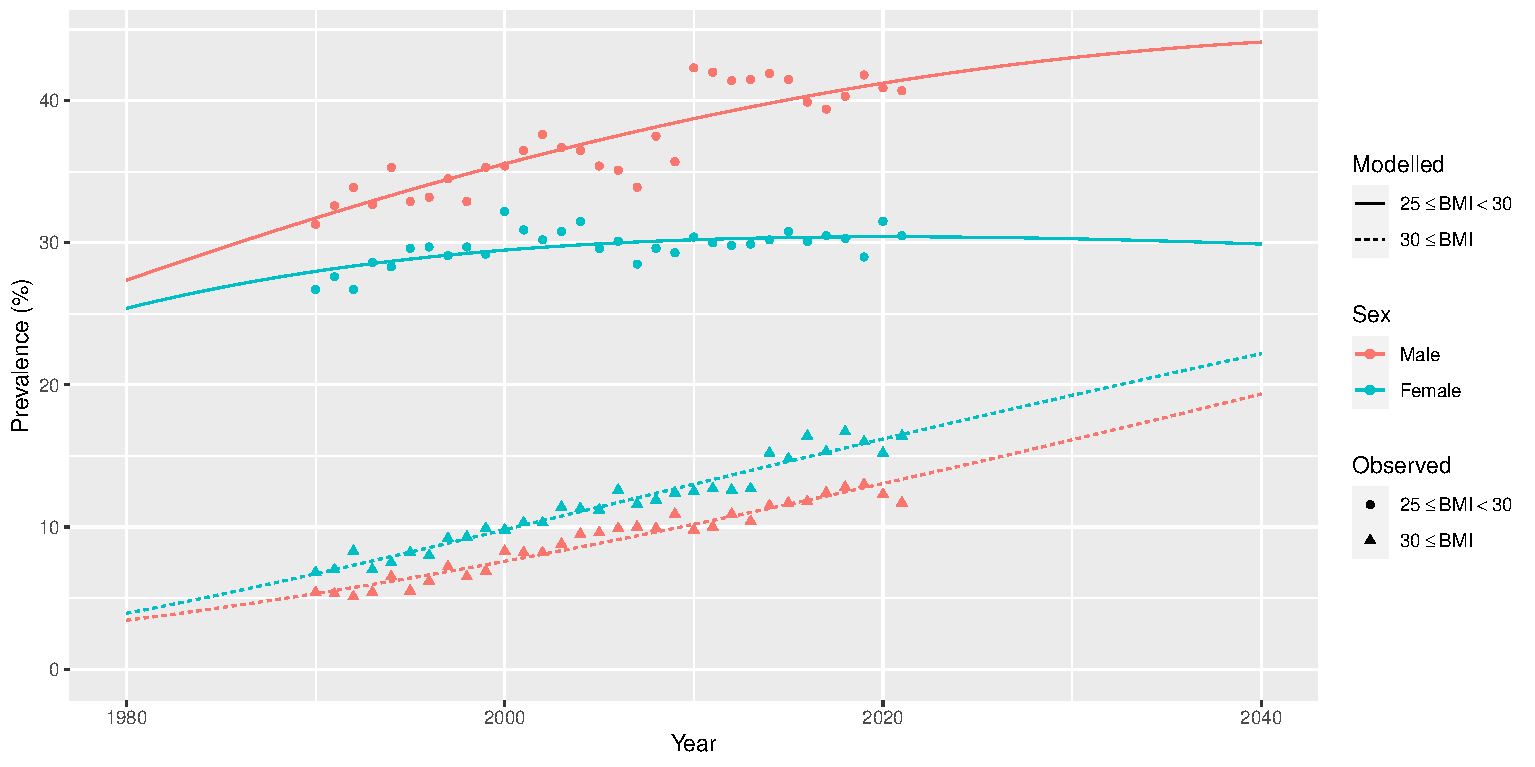
\includegraphics[width=0.99\textwidth] {"Figures/Historical-Trend.pdf"}
\caption{The observed and modelled prevalences of overweight and obesity by sex and year.}
\label{fig:Historical Trend}
\vspace*{-9pt}
\end{figure}

\section{Individual Trajectories}
\label{sec:Individual Trajectories}

\subsection{Approach}
\label{sec:Individual Trajectories/Approach}

At this stage, our risk factor model can only describe BMI at the population level. For many micro-simulations, such a model is already a useful building block. Then, simulated individuals can be assigned a percentile score indicating where they lie within the distribution which, in combination with their sex, level of education and age, produces a BMI value~\citep{McPherson2007, OECD2019}. As the individual ages throughout the simulation, this value can change while its relative position remains fixed. This is visualised as the fixed-percentile method in figure~\ref{fig:Individual Trajectories}.

We go one step further and allow for individuals to move within the population level distribution. Instead of looking at their percentile scores, we will examine and model their z-scores. Although the information contained in these two types of scores is equivalent, z-scores follow a normal distribution which make them easier to model. Our approach is to reduce the BMI values in our longitudinal data to z-scores following the transformation of equation~\ref{eq:Sinh-ArcSinh Transformation} and using values for $\mu$, $\sigma$, $\nu$ and $\tau$ which correspond to the individual's sex, level of education and age and to the calendar time of the measurement. Subsequently, we assume that individuals' z-scores follow stochastic trajectories over their lifetimes and that their BMI trajectories are those z-scores back-transformed to the original scale. Then, the union of all trajectories adheres to the shape of the population level distribution.

Individuals with the same sex, level of education and age can still have vastly different trajectories of BMI. Such heterogeneity is the result of various stochastic components which determine a life course and our model needs to be able to capture this. It may even be possible to identify subgroups with fundamentally different behaviour. For example, it has been suggested that fussy eaters follow different BMI trajectories from people who are less choosy~\citep{Herle2020}. This leads to growth mixture models where each subgroup's behaviour is determined by a separate model. However, we will assume all individual life course trajectories can be captured by the same mechanism, where three stochastic components form the source of individual variations.

The first component of these trajectories is the long-term effect. Heritability studies indicate a fairly strong genetic component to BMI, suggesting that individuals have a predisposition to belong to the upper- or lower percentiles of the distribution~\citep{Mathias2003, Goode2007, Ordonana2007}. Upbringing and other environmental causes may, too, have long-term effects, influencing someone's habits over their entire lifetime.

Fluctuations do occur however. Previous research has examined the temporal stability of BMI values~\citep{Wilsgaard2001, Ulmer2003, Juhola2011, Bayer2011}. These indicate slow changes over time, meaning values close in time correlate more than values measured further apart. Life events and new habits may influence eating- and exercise patterns, thereby affecting BMI, but it seems reasonable to assume that such effects eventually wane, making place for new habits. Modelling these dynamics correctly can be important when the relationship between a risk factor and a disease is simulated. Many such relationships are non-linear and an individual whose BMI fluctuates wildly can experience a different cumulative risk than one who follows a stable trajectory, even when their mean is similar~\citep{Murray2020}. That's why, in addition to the long-term effects, we also allow for medium-term effects.

Finally, BMI is subject to short-term fluctuations. Eating or drinking right before weighing yourself influences body weight and, therefore, BMI. Instrumental error originating from the measurement device also contributes. Whether these short-term fluctuations should be modelled as part of the generative process of BMI is up for debate. Instrumental error shows up in both cross-sectional and longitudinal data and increases the population variance~\citep{Biehl2013}. Such noise is best removed. Short-term effects with a physical interpretation, such as eating or drinking, or simply a short-lived new habit, might reasonably be considered a part of someone's BMI. Yet, these minor fluctuations have little causal influence on the onset of BMI-related diseases and are, for health modelling purposes, less relevant. Regardless, short-term fluctuations are estimated in our statistical analysis.

\subsection{Data}
\label{sec:Individual Trajectories/Data}

To understand how individuals move along typical trajectories and to distinguish between long-term, medium-term and short-term effects, we require longitudinal data with multiple measurements for each participant over a relatively long time. The Doetinchem Cohort Study provides such data. This study has followed a sex- and age stratified random sample from the population registers of the municipality of Doetinchem in the Netherlands for the past 30 years~\citep{Verschuren2008}. Its aim is to study lifestyle factors and biological risk factors on aspects of health. The participants underwent a health examination about every 5 years since 1987. A key feature of this panel is that characteristics such as weight and height were measured by research assistants instead of being self-reported. Table~\ref{tab:Doetinchem} provides some descriptive statistics of its latest round, focussing on the variables needed for our model which excludes some of the original data, removed in the cleaning process described in the online supplementary information~\citep{Bogaardt2023}.

\begin{table}[!h]
\tblcaption{Descriptive statistics of the Doetinchem dataset.}
{\mbox{\tabcolsep=18pt\begin{tabular}{@{}lcclr@{}}
\tblhead{& Number & Percentage & & Value\\[-9.5pt]}\\[-9.5pt]
Total & 3426 & 100\% & Minimum age & 45.9 \\
Male & 1606 & 46.9\% & Mean age & 64.0 \\
Female & 1820 & 53.1\% & Maximum age & 85.8 \\
Low education & 1491 & 43.5\% & Minimum BMI & 16.0 \\
Medium education & 1055 & 30.8\% & Mean BMI & 26.8 \\
High education & 880 & 25.7\% & Maximum BMI & 49.8 \lastline
\end{tabular}
\label{tab:Doetinchem}
}}
\vspace{-3mm}
\end{table}

The Doetinchem dataset is not completely representative of the Netherlands. For example, it lacks representation of ethnic subgroups and the study was not able to sample new cohorts from younger age categories~\citep{Picavet2017}. So, in addition to the Doetinchem data, we also make use of the Longitudinal Internet studies for the Social Sciences (LISS) panel~\citep{Scherpenzeel2010}. The LISS panel is a representative sample of Dutch individuals who participate in monthly Internet surveys. The panel is based on a true probability sample of households drawn from the population register. Households that could not otherwise participate are provided with a computer and Internet connection. A longitudinal survey is fielded in the panel every year, covering a large variety of domains including health, work, education, income, housing, time use, political views, values and personality. Table~\ref{tab:LISS} provides some descriptive statistics of its latest round which excludes some of the original data, removed in the cleaning process described in the online supplementary information~\citep{Bogaardt2023}.

\begin{table}[!h]
\tblcaption{Descriptive statistics of the LISS dataset.}
{\mbox{\tabcolsep=18pt\begin{tabular}{@{}lcclr@{}}
\tblhead{& Number & Percentage & & Value\\[-9.5pt]}\\[-9.5pt]
Total & 4630 & 100\% & Minimum age & 18.0 \\
Male & 2151 & 46.5\% & Mean age & 55.6 \\
Female & 2479 & 53.5\% & Maximum age & 104.0 \\
Low education & 1080 & 23.3\% & Minimum BMI & 15.8 \\
Medium education & 1643 & 35.5\% & Mean BMI & 25.9 \\
High education & 1907 & 41.2\% & Maximum BMI &49.6 \lastline
\end{tabular}
\label{tab:LISS}
}}
\end{table}

The LISS data were collected between 2007 and 2021, so they do not stretch over as long a period as the Doetinchem data. It also includes self-reported rather than measured values. On the other hand, it does contain a large group of young adults and is sampled with shorter time intervals, meaning both datasets complement each other well. The datasets were simply joined together before the analysis.

\subsection{Methods}
\label{sec:Individual Trajectories/Methods}

We model an individual's trajectory as a sequence of z-scores which indicate the positions relative to the population level distribution. Following our analysis in section~\ref{sec:Population Level Distribution}, we have a description of the BMI distribution using the sinh-arcsinh transformation and the four parameters $\mu$, $\sigma$, $\nu$ and $\tau$. These \mbox{parameters} depend on the individual's sex, level of education and age. From the analysis in section~\ref{sec:Historical Trend}, we also know how they depend on calendar time. Consequently, all BMI measurements from our longitudinal studies can be transformed using the specific parameters associated with the individuals'~characteristics and with the dates of the measurements. This removes any dependency on these variables from the z-scores.

The individual trajectories are assumed to contain long-term, medium-term and short-term effects. This can be described by a generalised autoregressive model. The long-term effects are then operationalised as a random intercept, which indicates the tendency to belong to the upper- or lower percentiles of the BMI distribution. In the fixed-percentile method, this random intercept is the only effect which determines the trajectories. Our model extends this method by including medium-term effects which are represented by a standard autoregressive process (AR1). This process assumes that, at each time period, a random shock occurs which either pushes the BMI z-score up or down. The effect of a shock decays exponentially over time, similar to how habits wax and wane. The overall effect is the sum of all previous shocks, which results in a meandering BMI value with temporal autocorrelation, as visualised in figure~\ref{fig:Individual Trajectories}. Short-term effects are modelled as additional, uncorrelated error representing daily fluctuations in weight. Note that no random slope is included. Models with these three components are described in detail in \cite{Diggle1988, Diggle1994} and \cite{Verbeke2000}.

Our model is described in equation~\ref{eq:Generalised Autoregressive Model}. Here, $Z_{i}$ is the vector of z-scores of individual~$i$ measured at $k$ time periods. This includes the three stochastic components of our model. $RI_i$ is the random intercept of individual~$i$, which has the same value for all measurements, and $J_k$ is the $k$-by-$k$ matrix with only ones. $AR1_i$ is the vector of $k$ correlated values, where the level of correlation between measurements is a function of the time between these measurements. Finally, $\epsilon_{i}$ is a $k$-vector of independent, random errors and $I_k$ is the identity matrix. This model was fit to the transformed longitudinal BMI data using the \textit{nlme} package in R~\citep{nlme2021, R2021}.

\vspace{-1mm}

\begin{equation}
\label{eq:Generalised Autoregressive Model}
\begin{array}{@{\ }rcl@{\ }}
Z_{i} & = & \beta_0 \, + \, \beta_1 \, \times \, age \, + \, RI_i \, + \, AR1_{i} \, + \, \epsilon_{i}\\[1.5mm]
RI_i & \sim & \mathcal{N}(0, \, \sigma_{intercept}^2 \, \times \, J_k) \\[-0.9mm]
AR1_{i} & \sim & \mathcal{N}(0, \, \Sigma) \ \ \text{where} \ \ \Sigma_{tt'} = \sigma_{correlated}^2 \, \times \, e^{-\frac{|t - t'|}{\tau_{AR1}}}\\[1.5mm]
\epsilon_{i} & \sim & \mathcal{N}(0, \, \sigma_{uncorrelated}^2 \, \times \, I_k)
\end{array}
\end{equation}

\vspace{1mm}

Our longitudinal data could, in principle, be used to estimate both a population level distribution and a historical trend of BMI. But this would only be useful if these data are representative of the Dutch population. We do not want to make this assumption and prefer to rely on the Public Health Monitor and the VZinfo datasets to model the population level distribution and historical trend of BMI. Whatever trend is contained in the longitudinal data, this should largely be removed when transforming the BMI values to z-scores because the transformation itself depends on calendar time via equation~\ref{eq:Population Level Distribution Parameters}. Nonetheless, if these data are not representative, this procedure need not result in values with zero mean and unit standard deviation; some bias may remain. Ultimately, we want a model which suits the entire population, so which produces true z-scores. A simple solution is to model the bias by including a fixed intercept and fixed slope in our statistical analysis, as shown in equation~\ref{eq:Generalised Autoregressive Model}. We are not interested in the values of this intercept and slope, but by including the terms, the other parameters are not compromised.

\subsection{Results}
\label{sec:Individual Trajectories/Results}

The estimated values, excluding the fixed intercept and slope, are listed in table~\ref{tab:Generalised Autoregressive Model Parameters}.

\begin{table}[!h]
\tblcaption{The parameters of the individual BMI z-score trajectories.}
{\mbox{\tabcolsep=18pt\begin{tabular}{@{}lcccc@{}}
\tblhead{& $\sigma_{intercept}^2$ & $\tau_{AR1}$ & $\sigma_{correlated}^2$ & $\sigma_{uncorrelated}^2$ \\[-9.5pt]}\\[-9.5pt]
Male & 0.5598 & 28.59 & 0.3961 & 0.04418 \\
Female & 0.6790 & 16.55 & 0.2886 & 0.03247 \lastline
\end{tabular}
\label{tab:Generalised Autoregressive Model Parameters}
}}
\vspace{-1mm}
\end{table}

The resulting covariance structure is also visualised in figure~\ref{fig:Covariance By Time Difference}, which shows the exponential decay and the asymptotes of the covariance between two BMI z-scores given their difference in time. Note that the three variances add up to one. Presented this was, the values for the three variances indicate the relative contributions of the long-term, medium-term and short-term effects.

\vspace{-4mm}

\begin{figure}[!h]
\centering
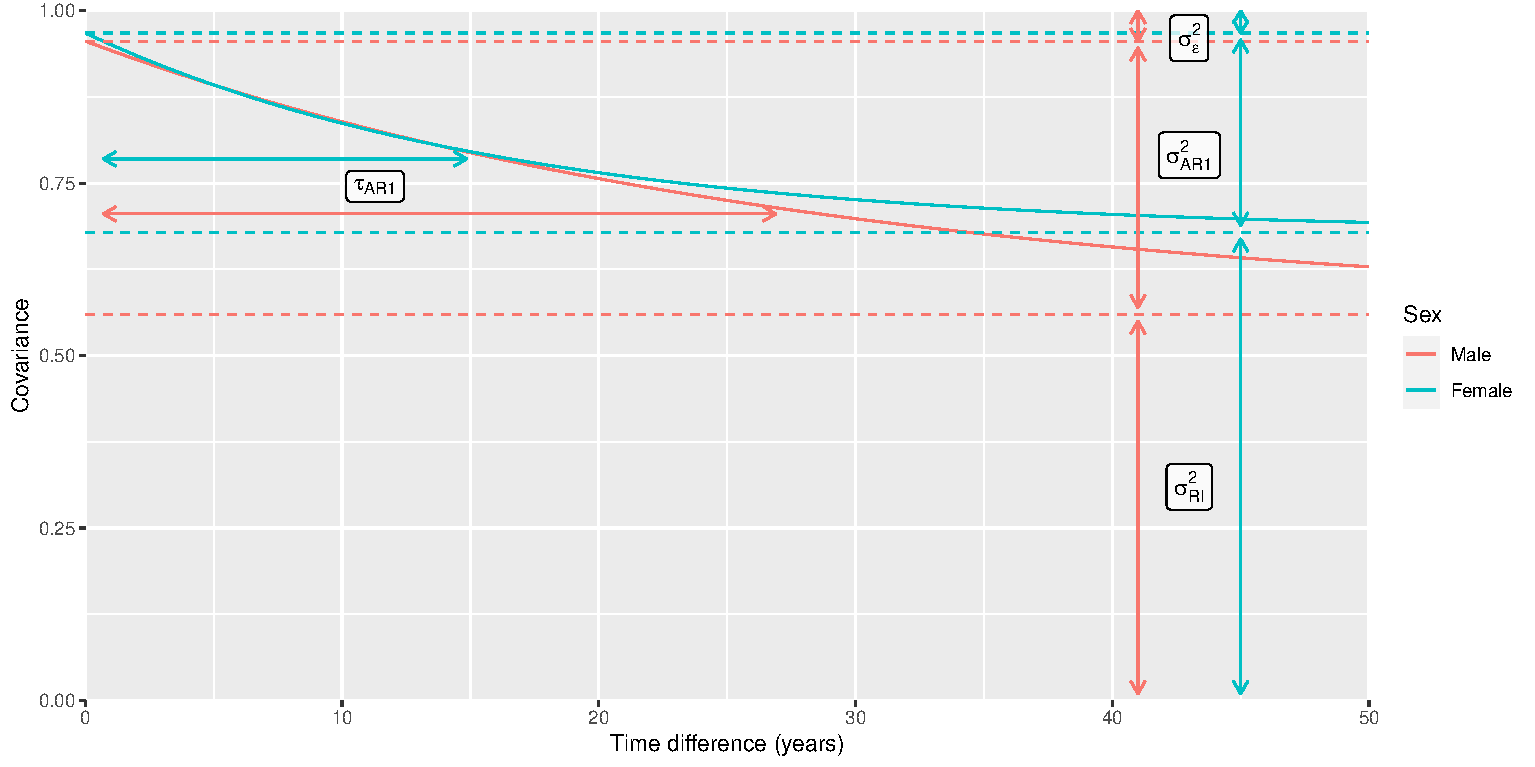
\includegraphics[width=0.82\textwidth] {"Figures/Covariance-By-Time-Difference.pdf"}
\vspace{-1mm}
\caption{The exponential decay in the covariance between two BMI z-scores given their difference in time.}
\label{fig:Covariance By Time Difference}
\vspace*{-9pt}
\end{figure}

\subsection{Internal Validation}
\label{sec:Individual Trajectories/Internal Validation}

To provide some feeling for the model, we can generate z-score trajectories and visually compare these to the data of a few individuals in the Doetinchem Cohort Study and LISS panel. Although it depends on the precise random samples which are drawn, figure~\ref{fig:Individual Z-Score Trajectories} shows that, on the face of it, the generated z-scores and the observed data are comparable. This give credence to our idea of modelling the transformed BMI values using a generalised autoregressive process with long-term, medium-term and short-term effects. By extension, we can conclude that the trajectories in figure~\ref{fig:Individual Trajectories} mimic realistic BMI trajectories.

\vspace{-4mm}

\begin{figure}[!h]
\centering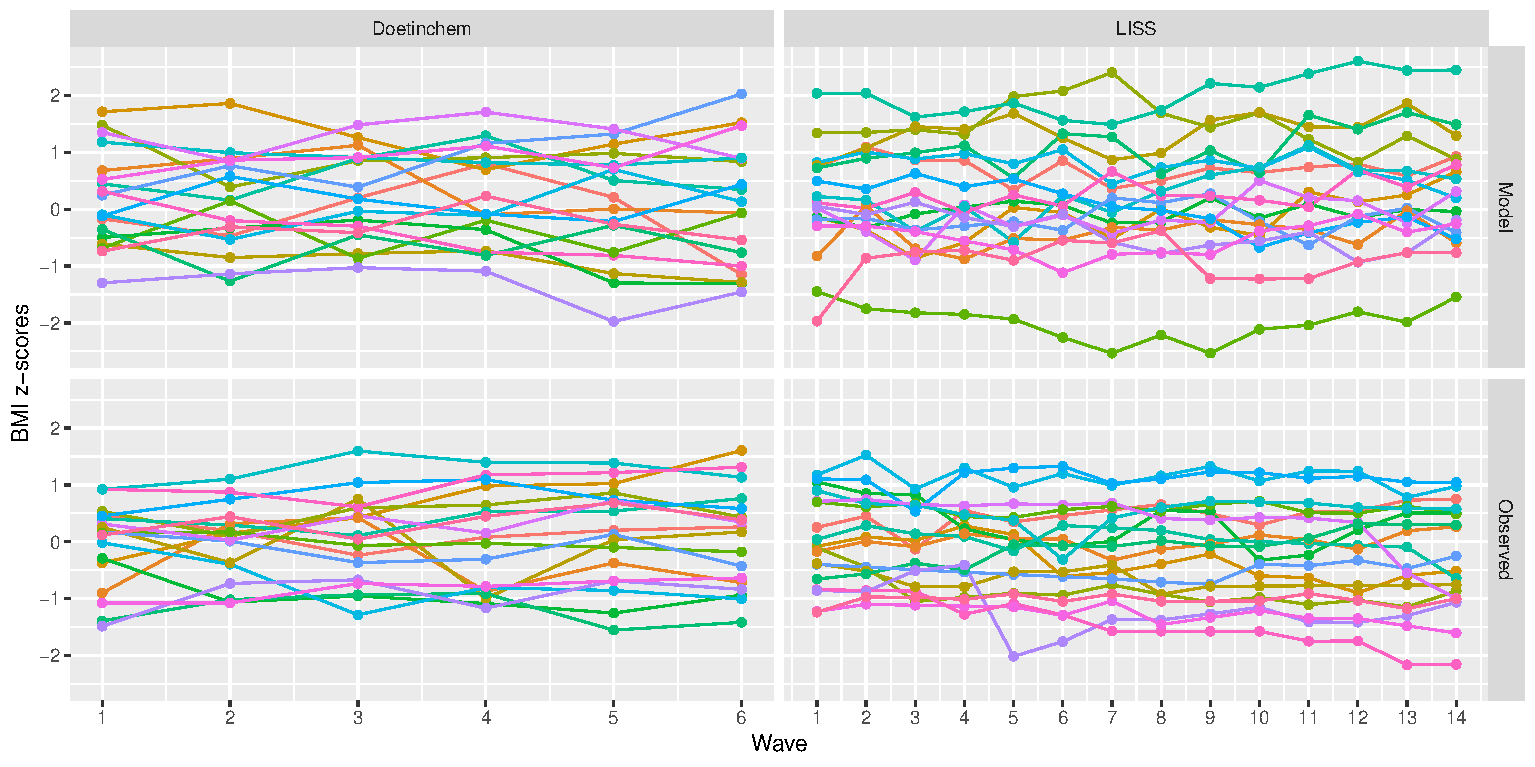
\includegraphics[width=0.99\textwidth] {"Figures/Individual-Z-Score-Trajectories.pdf"}
\vspace{-1mm}
\caption{A sample of observed and model-generated z-scores, coloured by individual, for Doetinchem and LISS.}
\label{fig:Individual Z-Score Trajectories}
\vspace*{-9pt}
\end{figure}

The model we have created is meant as a building block for micro-simulations. In a macro-simulation framework, a different modelling strategy is required, usually in the form of transition matrices. Estimating such matrices is not trivial and often simulations include no transitions at all~\citep{Hendriksen2015}. Others may include the smallest number of transitions between categories necessary to track changes in the population level distribution with age~\citep{VandeKassteele2012}. Our model can be converted to a transition matrix for application in a macro-simulation. The code to do so is available in the online supplementary materials~\citep{Bogaardt2023}. This retains much of the richness of our model, including the stratifications as well as the historical trends and additional fluctuations.

The ability to convert our model to a transition matrix naturally leads to another method to validate the results. We can first categorise all BMI values in the Doetinchem and LISS datasets into underweight, normal weight, overweight and obese. Then, every transition from one category to the next is counted and compared with the predicted transitions, shown in figure~\ref{fig:Transition Matrices}. The model approaches the observed transition rates between the four BMI categories but overestimates the fluctuations which occur for higher BMI values. This indicates that not all aspects of the life course trajectories are being reproduced, but that a large part of the relevant dynamics is indeed captured by our model. The differences seen between Doetinchem and LISS are mostly due to the different time intervals between measurements, where the Doetinchem data were recorded about every 5 years and the LISS data approximately every year.

\vspace{-5mm}

\begin{figure}[!h]
\centering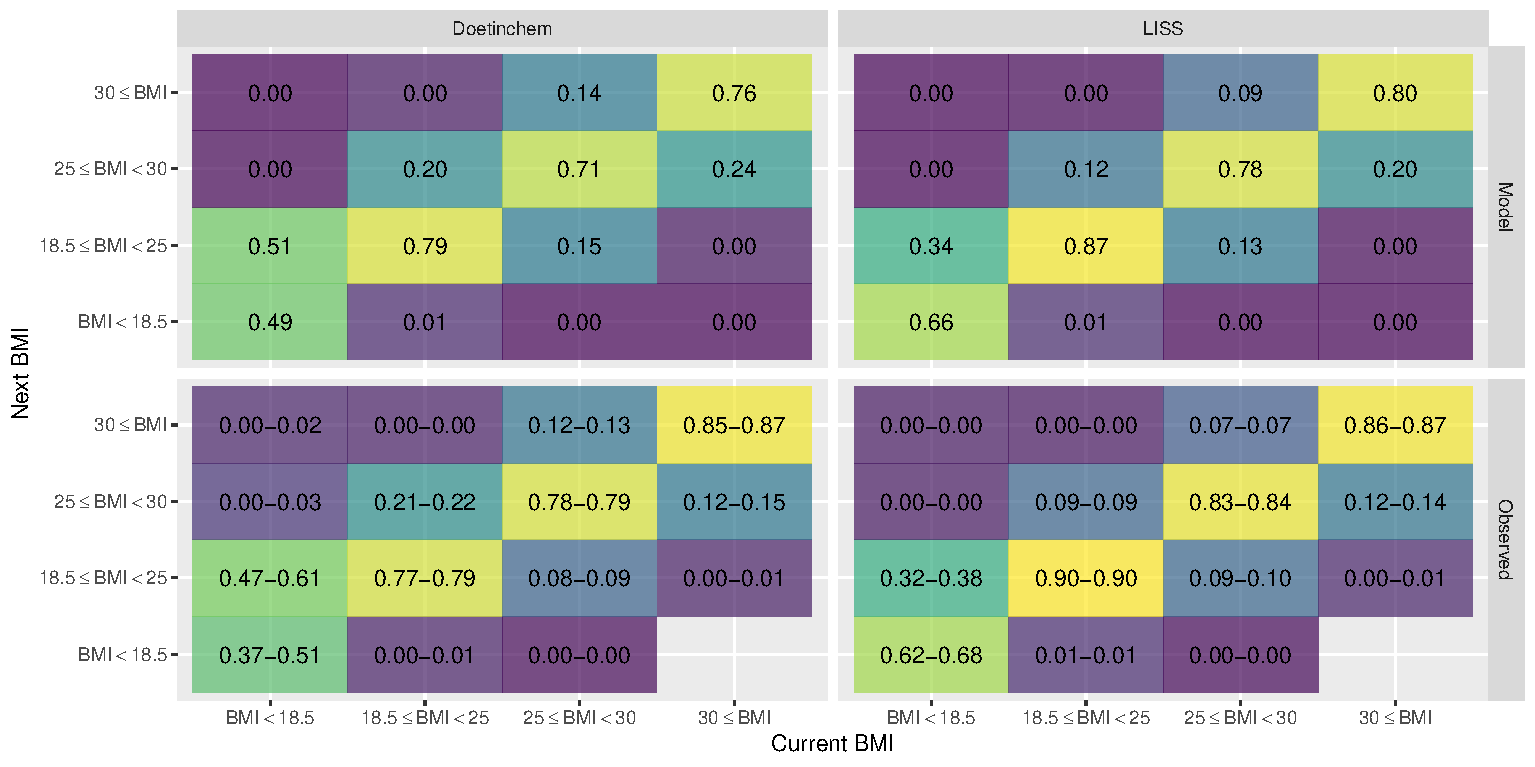
\includegraphics[width=0.99\textwidth] {"Figures/Transition-Matrices.pdf"}
\vspace{-2mm}
\caption{The observed and modelled transition matrix for the Doetinchem Cohort Study and the LISS panel.}
\label{fig:Transition Matrices}
\vspace*{-9pt}
\end{figure}

\vspace{-2mm}

\section{Discussion}
\label{sec:Discussion}

To summarise, we fitted a population level distribution of BMI, stratified by sex, level of education and age, to a cross-sectional dataset of the Netherlands in 2012. We added a trend using historical prevalences of overweight and obesity. Finally, we modelled individual trajectories as the z-scores of this distribution by making use of longitudinal data and a generalised autoregressive model with long-term, medium-term and short-term effects.

In section~\ref{sec:Population Level Distribution/Internal Validation}, we discussed the goodness of fit of the population level distribution and showed that our simple model produces representative population level distributions. Some limitations do remain. For one, the BMI values used to fit the model are self-reported. Previous research has shown that there can be a discrepancy between self-reported and measured BMI values and that individuals with a high BMI tend to underreport their weight~\citep{Olfert2018}. Although it may be possible to compensate for such discrepancies, we accept this as a weakness of our work and simply note that our model describes the population level distribution of self-reported BMI values.

Another limitation is that the cross-sectional data may be influenced by missingness due to BMI-related mortality. If a higher BMI leads to a higher mortality rate, the trajectories of the population's heaviest people will be censored. The resulting distribution then shows a lower mean BMI, especially at older ages. Whether this is an issue depends on the type of micro-simulation the model will be used in. If the simulation does not include a separate mortality process, describing the current BMI distribution of a country is best. If, however, mortality due to risk factors is added on top, then the BMI model should aim to describe the generative process. By obtaining information about the link between BMI and mortality, it becomes possible to compensate for this type of missingness. An easy method is to weight each participant in the cross-sectional data with the inverse of their BMI-related mortality rate before fitting the distribution.

In section~\ref{sec:Historical Trend/Internal Validation}, we discussed the goodness of fit of our historical trend and showed that by adding a linear trend to the $\mu$ and the $\sigma$ parameter, we can captures much of the recent change in the prevalences of overweight and obesity. Nonetheless, such a linear trend has limitations. For one, we are ignoring any interaction with education or age. The analysis in the supplementary materials indicated that this is a reasonable simplification~\citep{Bogaardt2023}. But more importantly, a linear trend predicts unrealistically low BMI values in the distant past and an ever increasing prevalence of overweight and obesity in the future. The ideal way to operationalise such a time effect would be to fit a sigmoidal function which asymptotically levels off to fixed values in both the distant past and the distant future. Due to limited data and our inherent ignorance of the future, however, a linear trend was fit. This entails that our model can only be valid for some time range around 2012, say, between 1980 and 2040.

A further limitation is that we are ignoring recent government actions to reverse the overweight and obesity trend in the Netherlands~\citep{VWS2018, VanRinsum2018}. Perhaps it is reasonable to assume that the increase in overweight and obesity has already started to slow down. If that is the case, our trend will not adequately predict the future and should have been fit on a more recent subset of the historical data. Alternatively, we could attempt to quantify the effects of these government actions and take those into account when extrapolating the trend.

In section~\ref{sec:Individual Trajectories/Internal Validation}, we discussed the goodness of fit of the generalised autoregressive model applied to the individual trajectories of z-scores. Although we have shown that our model fits the data reasonably well, these data contain intermittent missing values and dropouts. Our analysis assumes data are missing-at-random~\citep{Diggle1994, Verbeke2000}. This is probably a strong assumption as it is not unlikely that a higher BMI leads to a higher probability to miss a wave. In fact, BMI affects mortality rates and some of the dropout in our longitudinal data may be due to obesity-related death~\citep{Hoogenveen2000}. The fact that the Doetinchem and LISS datasets are not completely representative of the Netherlands is also a form of missing-not-at-random. In the ideal case, we would model the missing values using some mechanism which predicts intermittent missingness and dropout, but our solution to add a fixed intercept and slope may go a long way.

Another point to note is the linear dependence between the three stochastic components of the generalised autoregressive model. The random intercept, AR1 process and the uncorrelated error are not distinct mechanisms; an AR1 process with perfect temporal correlation leads to a random intercept, whereas a process with zero correlation leads to random noise. So, in a way, our model contains three distinct AR1 processes. As a result, small changes in the data may lead to relatively large changes in the parameters even though the resulting trajectories are nearly indistinguishable. The three stochastic components are, therefore, best interpreted together as part of a single mechanism, illustrated in figure~\ref{fig:Covariance By Time Difference}. In light of this, it may be concluded that the individual trajectories of males and females are quite similar.

Figure~\ref{fig:Individual Z-Score Trajectories} shows a few individuals who drastically gain- and lose weight over time. Such outlying transitions are not captured by our model. Contrarily, figure~\ref{fig:Transition Matrices} suggests our model slightly overestimates the amount of fluctuation which occurs for higher BMI values. Both observations can be true if there is a part of the population who have a particularly stable BMI and another whose BMI changes more rapidly. We had assumed the parameters listed in table~\ref{tab:Generalised Autoregressive Model Parameters}, which produce mildly fluctuating trajectories, hold true for the entire population. Future work could possibly extend the model using a growth mixture model where one subgroup follows fairly stable trajectories and another subgroup produces larger variations over time~\citep{Herle2020}. Regardless, our risk factor model already captures the majority of the heterogeneity within and between individual trajectories, and certainly more than the fixed-percentile method does. Modelling these dynamics correctly can be important when the relationship between a risk factor and a disease is simulated. Many such relationships are non-linear and an individual whose BMI fluctuates wildly can experience a different cumulative risk than one who follows a stable trajectory, even when their mean is similar~\citep{Murray2020}.

The risk of disease due to overweight is what drives governments to develop policies to reduce BMI~\citep{VWS2018}. Health simulations help to investigate what course of action is most fruitful by comparing a baseline scenario to an alternative scenario in which some preventive intervention has taken place. Interventions usually only apply to a subsection of the population where some criteria determine who is included. These criteria must be encoded into the health simulation. Our model allows for additional selection criteria based on the variations in an individual's BMI over time. Furthermore, it adds realism to the simulated selection procedure because, given the fluctuating BMI, an individual may satisfy the criteria one moment while fail to meet them the next, as occurs in real life.

Subsequently, the effect size of the proposed intervention must be analysed. Our model is a prediction model which describes the associations between sex, level of education, age, calendar time and BMI. We have not looked into the determinants of BMI nor claim any causal connection between variables. Nonetheless, in health simulations, causal connections are essential. When a lifestyle intervention is simulated, its effect on BMI must be modelled to be able to determine any health impact. In addition, assumptions must be made about if and how this effect wanes over time. It is tempting to assume the temporal autocorrelation found in our prediction model implies something about the speed at which intervention effects decay~\citep{Bayer2011}. We believe this to be unfounded; the immediate and lasting effects are best researched for every intervention separately~\citep{VanRinsum2018}.

Assuming it is clear what effect a preventive intervention will have, and on whom, this effect can be coded into the health simulation. Effects are frequently modelled by adjusting the parameters of the risk factor model. Although our model of BMI has many parameters which can be tweaked, we do not think all possible changes can be justified. Likely, altering the historical trend when predicting the future or changing an individual's random intercept can be defended. A better alternatively is to model the effect of interventions independent of the baseline risk factor model. For example, a hypothetical intervention may decrease BMI by one point initially and have a lasting effect of half a point. Such deviations can simply be added on top of a realistic BMI model such as ours. Policy effects aimed at an individual's life course may also be modelled as a decrease in the z-score. At the population level, such effects are visible because the union of all z-score trajectories would no longer produce a normal distribution with zero mean, but one with a slightly negative mean. Following the transformation shown in equation~\ref{eq:Sinh-ArcSinh Transformation}, the shape of the population level distribution of BMI would then be altered as well.

\section{Conclusion}
\label{sec:Conclusion}

We have create a risk factor model of BMI for micro-simulations which is able to faithfully describe the population level distribution, stratified by sex, level of education and age. It can also predict future trends in obesity as well as produce unique life course trajectories for individuals which seem plausible, but it does not capture extreme fluctuations, such as rapid weight loss. Our method is simple, tractable and a natural generalisation of the fixed-percentile method. The generic nature means it can be applied to data from various countries. Even when only cross-sectional data are available, it is probably valid to use the longitudinal parameters from our analysis to construct a country-specific model of individual BMI trajectories. Likewise, the method of fitting a flexible distribution at the population level and modelling longitudinal z-scores by a generalised autoregressive model could be applied to other continuous variables such as daily sugar intake, blood pressure or cholesterol levels. Finally, the risk factor model presented here can be simplified to a transition matrix for use in macro-simulations.

In future work, the model may be extended and generalised in multiple ways. First of all, a growth mixture model could be used to capture the variation between trajectories better, as previously discussed in section~\ref{sec:Discussion}. Secondly, the set of covariates can be expanded by any other predictor which has some association with BMI. The sole requirement is that this predictor is found in both the cross-sectional and the longitudinal data. Adding immigration-status may be helpful in the development of an accurate health simulation model to guide government policy~\citep{TenDam2023}. Additionally, the BMI trajectories of children and adolescents could be modelled. And finally, our generalised autoregressive model can be extended to multivariate outcomes to model multiple lifestyle characteristics. An example of previous work includes a model similar to ours that was used to simultaneously analyse CD4 T-cell and $\beta$-2-microglobulin measurements, both markers of AIDS~\citep{Sy1997}. One may also think of alcohol consumption and smoking, known to correlate with BMI~\citep{Chiolero2008, Traversy2015}. A model which predicts various risk factors simultaneously can be a great addition to the analysis of preventive interventions on lifestyle choices.

\vspace*{6pt}

\nocite{*}
\bibliographystyle{agsm}
\bibliography{A-Model-of-Individual-BMI-Trajectories}

\end{document}
